\chapter{Couplebreak}
V této kapitole se detailně seznámíme s modifikací pro KernelShark, která je schopna rozdělovat události a vytvářet pro ně záznamy KernelSharku. Tímto se zdvojí některé informace, což některým pluginům dovolí obejít omezení KernelSharku a být aktivní současně. Představeny budou cíle, analýza řešení, návrh a použití tohoto vylepšení. Konečnou částí pak bude kritika, ve které modifikaci zhodnotíme a představíme některá rozšíření.

\section{Cíle}
\begin{itemize}
    \item Podporované události dvou procesů dají vzniknout dvěma záznamům - původci a novému umělému záznamu.
    \item Modifikace bude navržena rozšiřitelně o další události.
    \item Nové záznamy budou patřit tomu procesu z páru, který předtím událost nevlastnil.
    \item Nové záznamy budou obsahovat odkaz na záznam s původní událostí.
    \item Nové záznamy budou splňovat rozhraní dotazů na záznamy KernelSharku. Tj. bude možné používat \texttt{kshark\_get\_*} funkce jako \texttt{kshark\_get\_pid}, nebo \texttt{kshark\_get\_info} apod.
    \item Nové záznamy bude možné filtrovat jednoduchým filtrem.
    \item Vylepšení bude možno zapnout a vypnout. Toto nastavení bude možné uložit do relací KernelSharku a načíst je z nich.
    \item Součástí vylepšení bude i zajištění kompatibility s pluginem sched\_events.
    \item Podporovány budou alespoň události sched\_switch a sched\_waking.
\end{itemize}

\section{Terminologie}
\begin{itemize}
    \item \emph{Couple/pár} je označení pro dva procesy, které sdílí nějakou událost. Například trasovací událost sched\_waking, kdy nějaký proces rozhodne o probuzení jiného procesu, přirozeně obsahuje dva procesy - probouzejícího a probouzeného. Páry se dají často rozdělit na procesy cílové a počáteční.
    \item \emph{Couplebreak událost} je fiktivní událost vytvořená Couplebreakem. Couplebreak momentálně vytváří pouze události cílové. Modifikace toto vyznačuje v sufixu jména události jako \uv{[target]}. Navíc každá taková událost v KernelSharku obsahuje ve svém jméně prefix \uv{couplebreak/}, podobně jako události plánovače úloh obsahují prefix \uv{sched/}. Couplebreak události mají speciální ID začínající na hodnotě \texttt{-10 000}, které se postupně vždy o 1 snižuje.
    \item \emph{Couplebreak záznam} je záznam vytvářený Couplebreakem pro Couplebreak událost. Významnou vlastností těchto záznamů je, že odkazují na záznam s událostí, kvůli které byla Couplebreak událost vytvořena.
    \item \emph{Origin/počáteční proces} je proces z páru, pro který existuje nějaká událost, se kterou tento proces ovlivní druhý proces z páru.
    \item \emph{Origin event/počáteční událost} je označení pro událost, která náleží počátečnímu procesu.
    \item \emph{Původní událost} je událost, při které se Couplebreak aktivuje a vytvoří Couplebreak událost.
    \item \emph{Target/cílový proces} je proces z páru, pro který existuje nějaká událost, která tento proces nějak ovlivní. 
    \item \emph{Target event/cílová událost} je označení pro událost, která náleží cílovému procesu.
    \item \emph{Vlastník události} je proces, během kterého událost nastala, resp. proces, v jehož grafu se událost objeví.
    \item Termíny \emph{(datový) stream, záznam, událost, relace} jsou převzaty z terminologie KernelSharku.
\end{itemize}

\section{Analýza}
Tato sekce se pokusí zachytit postup, kterým se dostaneme k implementaci řešení. Jedná se o techničtější analýzu než analýza z kapitoly \emph{Obecná analýza a stanovení požadavků}.

\subsection{Vytváření umělých záznamů}
Začněme s jádrem modifikace, rozdělování událostí. Musíme si rozmyslet, kde by bylo možné takovou akci provést. Z logiky fungování programu lze očekávat, že někde se musí události z Trace-cmd přetvořit na záznamy událostí pro KernelShark. Hledáme tedy funkci, která má toto na starosti. Podíváme se na cestu volání programu, když otevřeme nějaký soubor s trasovacími daty. Pak stačí postupovat hlouběji a hlouběji, dokud nenajdeme naši funkci, která nese název \texttt{get\_records}, která vytváří záznamy KernelSharku pro jeden stream. Právě zde KernelShark také vytváří umělé události pro situaci missed\_events, tedy události, které se staly, ale nebyly při trasování zachyceny. Ty KernelShark vytváří před nějakou jinou událostí a tyto umělé události jsou pak umístěny v grafu trasování a seznamu událostí před záznamy událostí, kvůli kterým byly vytvořeny. Navíc má KernelShark jedno hlavní pravidlo pro umělé události - jejich identifikátory musí být záporné. Nyní víme, jak správně vytvářet záznamy pro umělé události a jaká pravidla pro takové události má. Pokud se na funkci \texttt{get\_records} podíváme blíže, najdeme i místo, kde vytvářet umělé události tak, že budou v grafu i seznamu následovat po událostech, které způsobily jejich vznik, tj. původní události. Zde budeme vytvářet cílové události pro sched\_waking a sched\_switch. Druhá z událostí má navíc speciální část ve funkci, z čehož nám plyne i jak vynucovat chování pokud se jedná o nějakou specifickou událost.

Pokračujme tedy návrhem samotných Couplebreak událostí a jejich záznamů v KernelSharku. Identifikátory Couplebreak událostí zvolíme jako negativní hodnoty od hodnoty -10~000 a budou růst po jedné do zápornějších hodnot (tj. budou tvořit sekvenci -10~000, -10~001, -10~002, ...). S identifikátory budou nejspíš chtít pracovat i další části KernelSharku, nebo pluginy, proto je dáme do nového hlavičkového souboru \texttt{libkshark-couplebreak.h}. Identifikátory můžeme vytvořit jako konstanty, vytvoříme je tedy jako makra s číselnou hodnotou. Dále, záznamy pak vždy obsahují offset do souboru trasovacích dat, nicméně taková hodnota není pro umělou událost užitečná. Namísto toho splníme jeden z cílů nyní a pole \texttt{offset} bude obsahovat ukazatel na záznam původní události. Tak bude možné i využívat data původních událostí. Jelikož Couplebreak rozbíjí události mezi dvěma procesy, nastavíme nynějšího \uv{nevlastníka} původní události na vlastníka nové události. Naše události musejí být i jednoduše rozlišitelné pro člověka, všechny cílové tedy budou mít názvy ve formátu \texttt{couplebreak/\{původce\}[target]}, kde \{původce\} bude název události bez prefixu subsystému, kterému by náležela (například jenom část \uv{sched\_switch} z názvu \uv{sched/sched\_switch}). Specificky pro události sched\_waking budeme chtít změnit CPU, na kterém se událost stala, na CPU, kde bude proces doopravdy probuzen - detaily pro způsob jak toho docílíme vyřešíme později. Záznamy událostí označíme i jako plně viditelné jak v seznamu událostí, tak v grafu trasování. Ostatní informace můžeme zkopírovat z původní události, jelikož Couplebreak události nevyžadují další rozdíly a druhá podporovaná událost, sched\_switch, nemá nic, co by bylo zajímavé oddělené.

Nyní už víme, kde vytvářet události a co v nich má být. Vyřešme tedy jak je budeme vytvářet. Abychom mohli jednoduše rozšiřovat Couplebreak o další události v budoucnu, inspirujeme se tím, jak pluginy kreslí do grafu - v \texttt{get\_records} bude funkce, která přijímá konstruktory (specifikované signatury) a data, která se při vytváření využijí. Pak nám bude stačit vytvořit funkce specifikované signatury a předat jim data pro tvorbu událostí. Později lze definovat funkce pro další podporované události, pokud se přidají nové. 

Vytváření je skoro u konce. Vyřešíme už jen, jak nastavit správná CPU pro události sched\_waking[target]. Funkce, které volají \texttt{get\_records}, po práci této funkce setřídí vytvořené záznamy do jednoho pole, kde je vše uspořádáno podle času. Tímto se inspirujeme a vytvoříme setříděné pole, ve kterém následně najdeme správné CPU. Pole je nám poté k ničemu a zahodíme jej. Můžeme se zeptat, zdali nemáme nějaké dostupnější informace pro opravu CPU - odpověď je bohužel negativní. Události sched\_waking sice obsahují pole \texttt{target\_cpu}, ale to je pouze návrh. Operační systém a systémový plánovač úloh se může rozhodnout migrovat proces na nějaké jiné CPU a spustit ho až tam. Informaci o CPU, kde bude probouzená úloha opravdu spuštěna, je v události sched\_switch, která přepíná kontext nějakého CPU na probouzený proces. Informace je tedy vázána na víc než na původní návrh a pro její správnost je nutné prohledat události budoucí od původní sched\_waking.

\subsection{Stav Couplebreaku}
Couplebreak události je možné vytvářet, ovšem zatím se tomu tak děje vždy. To není v souladu s obecným požadavkem minimálního vlivu. Proto do datové struktury každého streamu přidáme proměnnou, která bude indikovat, zdali je Couplebreak ve streamu aktivní/zapnutý, či nikoliv. Zároveň si do streamu přidáme i počítadlo vytvořených typů Couplebreak událostí ve streamu a bitmasku, ve které budeme zaznamenávat, které Couplebreak události byly pro stream vytvořeny. Bitmasku implementujeme jako typ \texttt{int}. Bitmasku i počítadlo upravíme vždy pouze při prvním vytvoření Couplebreak událostí a nebo při inicializacích. Do funkce \texttt{get\_records} tedy přidáme kontrolu, zda je Couplebreak aktivní. Pokud ano, budeme vytvářet Couplebreak události. Počet událostí a bitmasku budeme v této funkci vždy znovu inicializovat. Výchozí hodnoty všech nových proměnných jsou 0, pro indikátor to znamená \texttt{false}.

\subsection{Úprava rozhraní datových streamů}
Aby se záznamy Couplebreak událostí mohly chovat jako obyčejné události, musíme dotazy na ně ošetřit v implementacích funkcí API streamu. Implementace očekávají možné vlastní umělé události, jako missed\_events události, takže i nastiňuje, kde by měl být kód, který řeší takové události. Tím se můžeme inspirovat. Rozhraní obsahuje několik funkcí, my si je dáme do seznamu a u každé si zapíšeme, zdali je něco potřeba měnit. Funkce mimo seznam nebyly pozměněny.
\begin{itemize}
    \item Získání PID ze záznamu pro Couplebreak nalezne nový v datových polích původní události.
    \item Získání jména události pro Couplebreak nové jméno vytvoří.
    \item Získání latence událostí pro Couplebreak požádá původní událost o tuto informaci.
    \item Získání obsahu datového pole \texttt{info} pro Couplebreak požádá původní událost o tuto informaci.
    \item Získání identifikátoru události přes její název pro Couplebreak vrátí jednu z konstant pro identifikátory Couplebreak událostí.
    \item Získání všech identifikátorů událostí nebude pozměněno. Kdyby se změnila tato implementace, mělo by to příliš široké následky ve zbytku kódu. Proto bude vytvořena nová funkce na získání identifikátorů všech Couplebreak událostí. Na získání opravdu všech identifikátorů přítomných událostí ve streamu bude doporučeno zkontrolovat Couplebreak a pokud je aktivní, tak si zažádat i o seznam jak normálních identifikátorů, tak o seznam Couplebreak identifikátorů.
    \item Výpis záznamu události pro Couplebreak nejprve vypíše název a PID procesu původní události a poté vypíše to samé, jako by se vypisovala původní událost.
    \item Získání dat z formátu události, tj. názvu, typu a hodnoty datového pole formátu události ze záznamu události, nebo z události samotné pro Couplebreak požádá původní událost o tuto informaci.
\end{itemize}

\subsection{Nové Couplebreak API}
Aby se nám s Couplebreakem lépe pracovalo a aby mohli některé jeho koncepty používat i jiné části kódu, dodáme s modifikací i malé API. V té budou pomocné funkce na získání často potřebných dat, hodnoty identifikátorů událostí a hodnoty jejich pozic v bitmaskách streamů. Dodáme následující funkce:
\begin{itemize}
    \item \emph{couplebreak\_get\_origin} - vrátí ukazatel na záznam původní události z pole \texttt{offset} předaného Couplebreak záznamu události.
    \item \emph{couplebreak\_origin\_id\_to\_flag\_pos} - vrátí pozici indikátoru v bitmasce datového streamu podle předaného identifikátoru původní události (tj. pro pozici indikátoru pro sched\_switch[target] předáme stream a identifikátor původní události v tomto streamu).
    \item \emph{couplebreak\_id\_to\_flag\_pos} - vrátí pozici indikátoru v bitmasce datového streamu podle předaného identifikátoru Couplebreak události.
    \item \emph{flag\_pos\_to\_couplebreak\_id} - vrátí identifikátor události podle předané pozice v bitmasce streamu.
    \item \emph{is\_couplebreak\_event} - určí, zdali je předaný identifikátor události identfikátorem nějaké Couplebreak události.
    \item \emph{get\_couplebreak\_event\_name} - vrátí jméno Couplebreak události, kterou určíme předáním jejího identifikátoru. Jméno je C-string a volající má na starosti tento řetězec dealokovat.
\end{itemize}

Všechny prvky tohoto API dáme do souborů \texttt{libkshark-couplebreak.c/h}. Tento soubor pak bude součástí knihovny \emph{libkshark}, k čemuž i upravíme CMake instrukce KernelSharku.

\subsection{Konfigurace}
\label{cbreak-cfg-subsec}
Couplebreak už teoreticky naplno funguje, ale musíme být schopni jej ovládat. K tomu si pořídíme konfigurační dialog, který přidáme do kódu k pomocným okénkům KernelSharku. Pro plnou kontrolu nad jeho obsahem budeme dědit přímo od \texttt{QDialog} a zbytek si postavíme pomocí Qt frameworku sami. Přidáme krátký vysvětlující text, aby uživatel věděl, na co klikl a co to umí. Poté přidáme zaškrtávací políčko pro zapínání Couplebreaku. Jelikož streamů může být otevřeno v jedné relaci více, budeme stavět políčka dynamicky podle počtu streamů. Abychom věděli, kterému streamu patří nějaké políčko, přidáme blízko něj popis ve formátu \texttt{Stream \#N}, kde N označuje identifikátor streamu. Naše rodičovská třída již zajišťuje tlačítka pro potvrzení, nebo zahození změn.

Co se interaktivity týče, tak propojíme potvrzující akci dialogu se změnou stavových proměnných Couplebreaku v příslušných streamech. Krom toho i donutíme KernelShark načíst všechna data znovu, aby se mohl Couplebreak projevit. Po datech také znovu načteme pluginy, aby mohly pracovat s novými daty. Tím dokážeme zapisovat provedené změny. Abychom ale také mohli zobrazovat aktuální konfiguraci, budeme pro každý stream kontrolovat, zdali je v něm Couplebreak zapnutý. Jestliže ano, tak zaškrtávací políčko předem zaškrtneme, jinak jej necháme nezaškrtnuté.

Konfigurační okénko se nezobrazí, pokud není načten alespoň jeden stream. Namísto toho se zobrazí chybová zpráva.

\subsection{Filtry}
KernelShark musí o Couplebreak událostech vědět alespoň v jednoduchých filtrech. Pokud by tomu tak nebylo, pak by při aplikaci jednoduchých filtrů nebyly Couplebreak události zahrnuty a KernelShark by je z grafu vyfiltroval. Přidáme tedy k dialogu pro jednoduché filtry funkci, která přidá do seznamu událostí i podsystém Couplebreak a události v něm. K tomu budeme pouze potřebovat získat všechny identifikátory Couplebreak událostí, což nám zajistí upravené stream API. Nakonec se stačí inspirovat kódem u obyčejného přidávání typů událostí do tohoto dialogu a poté můžeme přidat Couplebreak události.

Pokročilé filtry necháme stranou jako rozšíření modifikace. U těchto filtrů není žádný podstatný problém, jako u filtrů jednoduchých, tedy není tak nutné s nimi spolupracovat.

\subsection{Propojení s relacemi}
Ačkoliv není konfigurace Couplebreaku složitá, bylo by otravné ji při otevření relace vždy znovu nastavovat. Přidáme-li si čas navíc, který KernelShark musí strávit pro opětovné načtení dat, pak pro velká data bychom mohli čekat nepříjemně dlouho. Když si uložíme Couplebreak do relací, tak KernelShark bude potřebovat pouze jedno načtení a my se vyhneme opětovným konfiguracím.

Toto nejspíše bude ta nejjednodušší část implementace, jelikož bude stačit řídit se již existujícím ukládáním dat streamů do relačního souboru a poté uložit jeden bool, tj. indikátor zapnutého Couplebreaku. Nemusíme si ukládat nic dalšího, jelikož ostatní proměnné se vyplní při načtení dat. Při načítání pak budeme opět kopírovat to, co streamy obyčejně dělají, ale budeme jenom hledat hodnotu našeho indikátoru. Pro jednoduchost bude tato hodnota také boolovská, pod klíčem \uv{couplebreak}.

\subsection{Kompatibilita sched\_events s Couplebreakem}
Plugin sched\_events potřebuje měnit vlastníky sched\_switch událostí, aby mohl v grafech procesů správně vykreslovat rámečky pro latence. Se zapnutým Couplebreakem ve streamu, kde je plugin aktivní, tato potřeba odpadá. Plugin bude moci využívat ke kreslení události sched\_switch[target], které mají správné vlastníky pro potřeby pluginu. Nám tedy stačí detekovat Couplebreak, pokud je detekován, tak říci pluginu, ať se zajímá o cílové switch události a nemění vlastníky Couplebreak událostí. Tím jsme s pluginem hotovi.

\subsection{Zamítnutá alternativní řešení}

\subsubsection*{Couplebreak události pouze vizuální}
Jádrem tohoto přístupu bylo, že při vykreslování by se KernelShark pokusil zachytit podporovanou událost a nakreslit dva biny do grafu trasování. Nápad byl velmi rychle zamítnut, jelikož by toto byla operace pro každé vykreslení grafu, což má být pokud možno rychlá operace. Krom toho by vytváření prostoru pro bin bylo dle odhadů zbytečně složité a se záznamy by nebylo možno pracovat v jiných částech kódu, protože nic takového KernelShark nepodporuje.

\subsubsection*{Dynamické identifikátory událostí}
Kromě fixních identifikátorů pro Couplebreak události existoval i nápad, že budou negativními hodnotami identifikátorů původních událostí. Tento přístup byl ovšem zamítnut při návrhu dalších částí Couplebreak API, jelikož by bylo nutné vždy znát identifikátory původních událostí, což by byla práce navíc, která by i mohla obnášet přístup k souboru, což by byla další práce navíc.

\section{Vývojová dokumentace}
Tato sekce hodlá předat čtenáři strukturu modifikace, podle které se lze v modifikaci orientovat. Zároveň pak dodá krátký návod pro vývojáře, kteří by chtěli s Couplebreakem pracovat ve svých pluginech či změnách pro KernelShark.

\subsection*{Názvy}
Krátkou část ještě věnujme názvům přidaných prvků v kódu. Ačkoliv je každá změna ohraničena komentáři, které ji vyznačují, jsou prvky pojmenovány tak, aby čtenář ihned poznal, že něco souvisí s touto modifikací. To je dosaženo tím, že součástí jména nových prvků je řetězec \texttt{couplebreak}, často jako prefix. Tak je tomu v novém API, ale i v čistě implementačních funkcích, pokud nebyla značka v ohraničujícím komentáři sama ohraničena uvozovkami (viz vysvětlení ohraničujících komentářů \ref{comment-style}).

\subsection{Struktura modifikace}

Modifikaci rozdělíme na moduly. Modifikace obsahuje několik částí, které ji různě integrují do existujících modulů KernelSharku. Jejich seskupením do \uv{integračního modulu} bychom přišli o lepší rozdělení, proto budou integrační části samostatnými moduly. Pro detailnější informace a implementační detaily je doporučeno prohlédnout si samotný kód a technickou Doxygen dokumentaci KernelSharku, jejíž novou součástí jsou i části o modifikaci.

Ke každému modulu připíšeme i soubory, ve kterých je modul implementován, a prvky modulu jako veřejné funkce, makra, či veřejné třídy. Prvky mimo hlavičkové soubory, nebo označeny za privátní pro třídu jsou brány jako implementační detaily a nebudou zde popsány (lze je najít uvnitř souborů modulu).

V kódu modifikace používá značku \texttt{COUPLEBREAK} v ohraničeních změn.

\subsubsection*{Couplebreak API}
Tento modul dodává nové konstanty a funkce, hlavně pro získávání informací. V souborech modulu jsou definovány identifikátory pro jednotlivé Couplebreak události, pozice indikátorů v bitové masce aktivních Couplebreak událostí ve streamech a funkce Couplebreak API, aby další kód (například pluginy) mohl s Couplebreakem pracovat.

\begin{itemize}
    \item \textbf{Soubory:} libkshark-couplebreak.h/c
    \item \textbf{Makra:}
    \begin{itemize}
        \item \emph{COUPLEBREAK\_SST\_ID} - identifikátor události sched\_switch[target].
        \item \emph{COUPLEBREAK\_SWT\_ID} - identifikátor události sched\_waking[target].
        \item \emph{COUPLEBREAK\_SSWITCH\_FPOS} - pozice indikátoru pro událost sched\_switch[target] v Couplebreak bitmasce ve streamu.
        \item \emph{COUPLEBREAK\_SWAKING\_FPOS} - pozice indikátoru pro událost sched\_waking[target] v Couplebreak bitmasce ve streamu.
    \end{itemize}
    \item \textbf{Funkce:}
    \begin{itemize}
        \item \emph{couplebreak\_get\_origin} - vrátí záznam původní události záznamu Couplebreak události.
        \item \emph{couplebreak\_origin\_id\_to\_flag\_pos} - vrátí pozici indikátoru uvnitř bitmasky Couplebreaku datového streamu z identifikátoru události, ke které by Couplebreak vytvořil Couplebreak událost.
        \item \emph{couplebreak\_id\_to\_flag\_pos} - vrátí pozici indikátoru uvnitř bitmasky Couplebreaku datového streamu z identifikátoru Couplebreak události.
        \item \emph{flag\_pos\_to\_couplebreak\_id} - vrátí identifikátor Couplebreak události z pozice indikátoru v bitmasce Couplebreaku datového streamu.
        \item \emph{is\_couplebreak\_event} - zjistí, zdali je daná událost Couplebreak událostí.
        \item \emph{get\_couplebreak\_event\_name} - vrátí jméno Couplebreak události z identifikátoru Couplebreak události. 
    \end{itemize}
\end{itemize}

Tento modul je také důvodem změny souboru \emph{CMakeLists.txt} v adresáři zdrojového kódu KernelSharku, jelikož soubory jej obsahující jsou nové.

\subsubsection*{Konfigurace}
Modul se zajímá hlavně o GUI okénko pro konfiguraci Couplebreaku a aplikaci změn provedených v tomto okně na streamy, kterých se to týká. Kvůli této povinnosti tento modul hlavně komunikuje s modulem integrace do datových streamů. V souborech modulu byly do hlavního okna přidány grafické elementy pro ovládání Couplebreaku přes GUI.

\begin{itemize}
    \item \textbf{Soubory:} KsMainWindow.hpp/cpp, KsWidgetsLib.hpp/cpp
    \item \textbf{Třída:} nová třída \emph{KsCouplebreakDialog} pro okénko konfiguračního dialogu Couplebreaku.
\end{itemize}

\subsubsection*{Integrace do datových streamů}
Couplebreak se v tomto modulu spojuje s datovými streamy KernelSharku a funkcemi, které je využívají. Dodává nové funkce, upravuje implementace funkcí starých, aniž by porušil jejich původní funkcionalitu, a přidává proměnné do datových struktur streamů správě stavu Couplebreaku.

\begin{itemize}
    \item \textbf{Soubory:} libkshark.h/c, libkshark-tepdata.c
    \item \textbf{Datové položky} v \texttt{kshark\_data\_stream}:
    \begin{itemize}
        \item \texttt{couplebreak\_on} - indikátor zapnutého či vypnutého Couplebreaku ve streamu.
        \item \texttt{n\_couplebreak\_evts} - počet vytvořených typů Couplebreak událostí.
        \item \texttt{couplebreak\_evts\_flags} - bitmaska, která zaznamenává, které typy událostí jsou ve streamu přítomné.
    \end{itemize}

    Nedoporučuje se při běhu KernelSharku měnit jakoukoliv z položek výše, podobně jako se nedoporučuje měnit například počet originálních zaznamenaných událostí ve streamu, \texttt{n\_events}. Modifikace nemá definované chování, pokud se tyto položky změní. Čtení není nijak omezeno.

    \item \textbf{Rozšíření rozhraní:} nová funkce v rozhraní \emph{get\_couplebreak\_ids} datových streamů. Má vlastní nový typ funkce, \texttt{stream\_get\_couplebreak\_ids\_func}.
\end{itemize}

\subsubsection*{Tvoření záznamů Couplebreak událostí}
Modul má na starost vytvářet záznamy Couplebreak událostí, opravovat jejich data, a spojovat je s původními událostmi. Modul řeší čistě implementaci a nelze s ním komunikovat skrze veřejná rozhraní.

\begin{itemize}
    \item \textbf{Soubor:} libkshark-tepdata.c
\end{itemize}

\subsubsection*{Integrace do jednoduchých filtrů}
Zde jsou upraveny jednoduché filtry tak, aby věděly o Couplebreak událostech a ty mohly být filtrovány. Úpravy se týkají GUI pro jednoduché filtry. Modul řeší čistě implementaci a nelze s ním komunikovat skrze veřejná rozhraní.

\begin{itemize}
    \item \textbf{Soubory:} KsMainWindow.cpp, KsWidgetsLib.hpp/cpp
\end{itemize}

\subsubsection*{Integrace do relací}
Tento modul se stará o ukládání Couplebreaku do relačních dat streamů KernelSharku a načítání Couplebreaku z relací. Modul řeší čistě implementaci a nelze s ním komunikovat skrze veřejná rozhraní.

\begin{itemize}
    \item \textbf{Soubor:} libkshark-configio.c
\end{itemize}

\subsection{Úpravy mimo logiku modifikace}

\subsubsection*{Spolupráce sched\_events s Couplebreakem}
Rozšíření oficiálního pluginu sched\_events, dovoluje pluginu používat Couplebreak události a otevírá tak kompatibilitu pro další pluginy. Rozšíření je obsaženo v souboru \emph{sched\_events.c}.

\subsubsection*{Nová funkce v \emph{KsUtils} jmenném prostoru}
Funkce \emph{getCouplebreakIdList} vrátí volajícímu seznam identifikátorů všech Couplebreak událostí přítomných v daném streamu. Použito v modulu \emph{Integrace do jednoduchých filtrů}. Úprava obsažena v souborech \emph{KsUtils.hpp/cpp}.

\subsection{Vyvíjení pro KernelShark s Couplebreakem}
Modifikace se snaží být nerušivou součástí KernelSharku. Pokud budeme někdy chtít dále vyvíjet pro KernelShark, tak lze naše změny třeba nejprve navrhnout pro KernelShark bez aktivního Couplebreaku a až poté se pokoušet o integraci, pokud je nutná. Většinou by pak měl nový kód kontrolovat zda je Couplebreak aktivní přes proměnné ve streamu a měnit chování podle této informace. Samozřejmě existují i vylepšení, pro která nemá taková kontrola smysl, například rozšíření relací o nový datový formát - zde je nutné ukládat data Couplebreaku (alespoň zda byl ve streamu aktivní).

Vývojář pluginů pak může využít Couplebreak API a také kontrolovat přítomnost této modifikace ve streamu a dál tato data využívat. Modifikace by pak měla být respektována vždy, kdy se se očekává nějaký sled událostí a Couplebreak nějakou z nich dokáže dělit. Couplebreak ale může i pomoci s vytvořením kompatibility pro nějaké pluginy. Příkladem mohou být pluginy sched\_events a \emph{Naps}\ref{nappin}. Oba z pluginů potřebují měnit procesy vlastnící nějaké události, aby mohly kreslit své tvary do grafu jednoho procesu. Pokud jsou oba pluginy aktivní bez zapnutého Couplebreaku, tak buď kreslí mezi špatnými záznamy, nebo na špatných místech. Oba totiž pohnuly se záznamy a narušili tak očekávání druhého z nich. S Couplebreakem nemusejí se záznamy hýbat, jelikož pro své potřeby si mohou vybrat záznamy od Couplebreaku.

V nižších sekcích jsou popsány situace, se kterými se vývojáři nejspíše nejčastěji setkají při práci s Couplebreakem.

\subsubsection*{Dotazy na záznamy KernelSharku}
Každá funkce v rozhraní dotazů na záznamy KernelSharku může být používána jako dříve, i s Couplebreak událostmi. Pro Couplebreak většinou taková funkce bude pracovat s daty původního záznamu. Druhou možností je, že Couplebreak vytvoří požadované hodnoty na místě. To je hlavní rozdíl oproti normálním záznamům událostí, jelikož ty takovou hodnotu získávají ze souboru s trasovacími daty.

Například: zavolám-li \texttt{kshark\_find\_event\_id}, tak KernelShark zachytí jméno hledané události. Během průběhu funkce, která má na starosti získání jména z originálních trasovacích dat, Couplebreak předá kontrolu jiné funkci. Ta na základě přítomnosti Couplebreaku ve streamu buď vrátí správný identifikátor, nebo vrátí neplatný identifikátor, nebo předá kontrolu původní funkci, pokud nebylo hledané jméno součástí jmen událostí Couplebreaku.

\subsubsection*{Záznamy Couplebreak událostí}
Couplebreak události jsou přidány za běhu programu a nemohou nijak kontrolovat \uv{původní data}, například původní název procesu, kterému událost patří. Dotazy na taková data jsou tak buď nasměrovány na záznamy událostí, kvůli kterým vznikly, nebo vytvořením dat nanovo, viz předchozí sekce.

Toto je způsobeno tím, co je v datech záznamů Couplebreak událostí, speciálně v jejich poli \texttt{offset}. Tam již není offset do trasovacího souboru, nýbrž ukazatel na původní záznam události. Z toho také vychází, že toto pole se nikdy nesmí pro záznamy Couplebreak událostí měnit. Kromě tohoto pole je zakázáno i jakkoliv měnit pole \texttt{event\_id}, jelikož pro takový záznam je tato změna nevratná. Pokud jakékoliv z těchto dvou polí bude změněno, chování takového záznamu je nedefinováno, záznam lze považovat za rozbitý a již neobsahuje Couplebreak událost.

\section{Uživatelská dokumentace}

\subsection{Instalace}
Couplebreak je součástí zdrojového kódu KernelSharku a je ve více souborech, některé z nich jsou nové. Proto byl upraven soubor sestavovacích instrukcí CMakeLists.txt. Pokud již máte nainstalovaný KernelShark, tak jej nainstalujte znovu, je nutné, aby se sestavil i s novými soubory. Instrukce k instalaci KernelShark dodává sám KernelShark a jsou také popsány v kapitole o něm \ref{kap-kernel-shark}.

\subsection{GUI}

Uživatel GUI KernelSharku musí Couplebreak zapnout, modifikace je ve výchozím nastavení vypnutá. Stačí kliknout na nové tlačítko \texttt{Couplebreak Settings} v submenu \texttt{Tools} v menu KernelSharku, viz obrázek \ref{cbreak-tools}. Mělo by být umístěno pod tlačítkem \texttt{Record}. Po kliknutí se zobrazí konfigurační okénko, ve kterém se dá Couplebreak zapnout pro každý z otevřených streamů zvlášť, viz obrázek \ref{cbreak-multiconf}. Součástí okénka je i krátký vysvětlující text této modifikace, tlačítko \texttt{Apply} na použití vybrané konfigurace a tlačítko \texttt{Cancel} na zavření okénka bez provedení změn.

\begin{figure}[p]\centering
    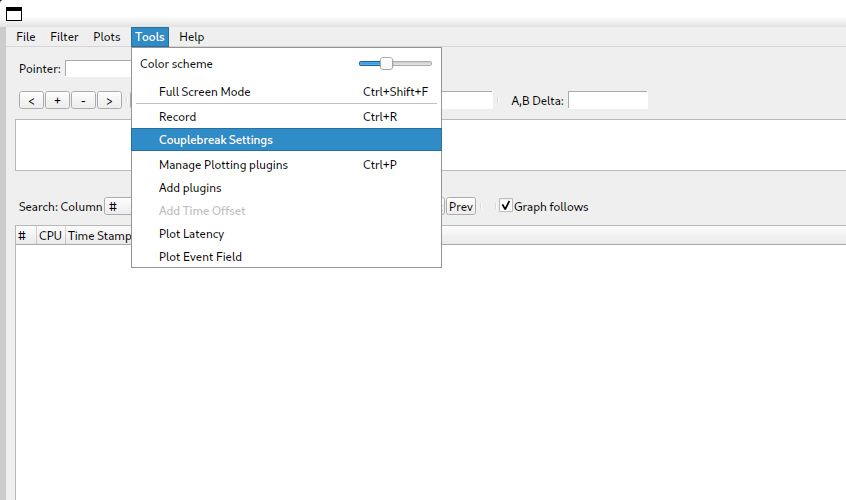
\includegraphics[width=140mm]{img/Modifikace/modif-couplebreak-tools}
    \caption{Submenu tools s modifikací tlačítkem pro konfiguraci Couplebreaku.}
    \label{cbreak-tools}
\end{figure}

\begin{figure}[p]\centering
    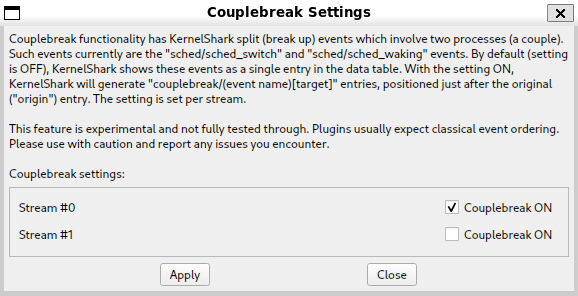
\includegraphics[width=140mm]{img/Modifikace/modif-couplebreak-multiconf}
    \caption{Dva streamy jsou otevřené, v jednom z nich je aktivní Couplebreak.}
    \label{cbreak-multiconf}
\end{figure}

Zaškrtnutím políčka pro nějaký stream v konfiguračním okénku a následným použitím této konfigurace se data ve streamech načtou znovu. Toto také donutí pluginy aktivní v dotyčných streamech, aby se znovu načetly. Pluginy si tak mohou obnovit svůj kontext a použít nová data (tj. s novými záznamy Couplebreak událostí).

Záznamy Couplebreak událostí mohou být filtrovány jednoduchým filtrem stejně jako ostatní události, viz obrázek \ref{cbreak-filter}. Nelze je filtrovat pomocí pokročilých filtrů, ty nejsou podporovány. Záznamy jsou viditelné v seznamu událostí a i v grafu. Je možné, že budou zakrývat záznam své počáteční události, nebo budou naopak zakrývány takovým záznamem. Z hlediska rozlišení událostí to není velký problém, obě události jsou v podstatě to samé, jenom rozdělené. Pro vybrání zakrytého záznamu je pak nejjednodušší jej vybrat v seznamu událostí.

\begin{figure}[p]\centering
    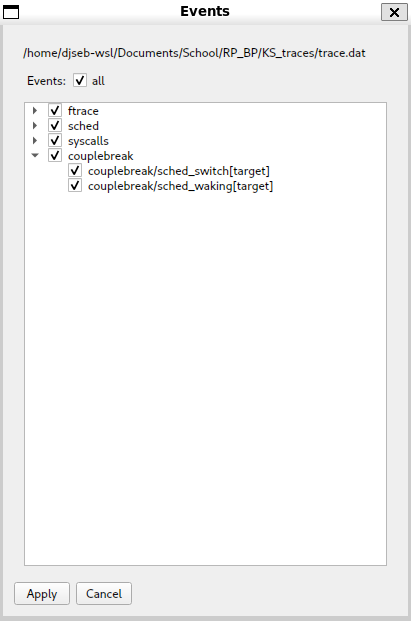
\includegraphics[width=140mm]{img/Modifikace/modif-couplebreak-filter}
    \caption{V jednoduchém filtru lze vybírat i Couplebreak události.}
    \label{cbreak-filter}
\end{figure}

\section{Bugy a chyby}

Záznamy Couplebreak událostí by se neměly účastnit kreslení obdélníků mezi záznamy v grafu, jelikož nepředstavují opravdovou práci, nýbrž důsledek práce někde jinde. KernelShark ale nemá jak rozlišit tyto záznamy a obdélníky se kreslí i pro ně. Vylepšení \emph{NoBoxes} se snaží toto chování opravit, nicméně neumí to dokonale.

Během vývoje KernelSharku dvakrát spadl při opravě CPU pro sched\_waking[target] záznamy. Ačkoliv bug se již dlouho neobjevil, nebyl ani explicitně opraven. Pokud by KernelShark spadl při načítání trasovacích dat, je možné, že příčinou byl Couplebreak.

\section{Rozšíření}
Tato sekce představí některá rozšíření, která by modifikaci zjednodušila, nebo by dodala nové funkce. Upozorňujeme, že se mohou objevit rozšíření, která upravují čistě implementaci, například zlepšují čitelnost kódu - u těchto se očekává znalost kódu vylepšení. Takové části budou vždy označeny v první větě jejich sekce.

\subsubsection*{Podpora více událostí}
Přirozeným rozšířením této modifikace by bylo rozšíření Couplebreaku o více událostí, případně i o vytváření nějakých počátečních událostí. Existující kód Couplebreak událostí a všeho, co s jich týká, by měl dostatečně nastínit, jak postupovat při takových změnách.

\subsubsection*{Optimalizace průchodů daty při opravě CPU pro sched\_waking}
Couplebreak ve své stávající podobě donutí nasbíraná data, aby byla setříděna dle CPU a času do nějakého pole, ve kterém poté vyhledá konečná CPU pro probouzené události, tzv. opraví CPU. Stejné pole později vytváří ale i další funkce, které jsou zavolány po naší opravě. Vytváříme tedy pole, které poté zahodíme, ale po chvíli je vytvořeno znovu. Toto rozhodně představuje prostor pro optimalizace.

První možnou optimalizací je prosté neopravování CPU cílových událostí. Zkrátka volání opravy neprovedeme. Tím ale také přijdeme o informaci, kde nakonec byl proces probuzen. Je to ovšem nejjednodušší řešení.

Druhou možností je použít trik podobný hledání záznamů zásobníku v pluginu \emph{Stacklook}. Vytvořili bychom plugin, který cílovým událostem CPU opraví v jednom průchodu při prvním pokusu o kreslení a dále se nevolá, pokud není plugin načten znovu. Nápad to není špatný, ale bylo by nutné pak řešit situace, kdy by některé jiné pluginy nebo části KernelSharku mohly očekávat původní CPU.

Třetí možností je ponořit se vnitřností KernelSharku a upravit místa, kde se pole vytváří a místa, kde zanikají. Pokud bychom opravili CPU, tak bychom si možná mohli na pole uschovat ukazatel a nějakým způsobem ho předat funkcím, které by pak nemusely vytvářet nové setříděné pole. Toto by byla čistá optimalizace a nebylo by nutné oddělovat opravy CPU od Couplebreaku.

\subsubsection*{Funkce \texttt{get\_*\_event\_ids} a širší podpora pro umělé události}
Couplebreak přidal \texttt{get\_couplebreak\_evt\_ids} (\uv{Couplebreak} funkce) do rozhraní streamu. Vytvořena byla proto, že úprava \texttt{get\_all\_event\_ids} (\uv{all} funkce) pro spolupráci s Couplebreakem by způsobila příliš mnoho úprav chování v místech, kde byla použita. Tato použití někdy vůbec nepotřebují o umělých událostech vědět.

S \uv{Couplebreak} funkcí je ale funkcionalita \uv{all} funkce narušena - nyní už nevydá všechny události ve streamu, nýbrž jen všechny události, které nejsou vytvořeny Couplebreakem. Bylo by proto lepší, kdyby \uv{all} funkce byla alespoň přejmenována, aby lépe odrážela svou práci, například na \texttt{get\_all\_original\_event\_ids}. Poté bychom i mohli dodat funkci, která by vrátila opravdu všechny události. Dobré by pak bylo projít celý kód KernelSharku a rozhodnout zdali jsou na místech použití \uv{all} funkce potřeba všechny události, nebo pouze originální události.

Celkově by bylo hezké dodat KernelSharku obecnou podporu pro práci s umělými událostmi, nejen pro události od Couplebreaku. Ten je sice jediným výrazným producentem umělých událostí, ale nemusí tomu tak být napořád, mohou přibýt další vylepšení, která budou umělé události využívat.

\subsubsection*{Rozdělování pouze některých událostí}
Možným rozšířením je rozdělování pouze některých událostí, které bychom si vybrali v konfiguraci. Tím by bylo rozdělování jemnější. Nicméně by také bylo nutné refaktorovat části, které kontrolují aktivní Couplebreak, například pokud by nás zajímalo jenom to, zdali se rozdělují události typu sched\_switch. Zároveň by toto znamenalo indikátory pro každou událost, na což by mohla být opět použita bitmaska.

\subsubsection*{Podpora pokročilých filtrů}
Couplebreak události mohou být filtrovány jen pomocí jednoduchých filtrů. Ale bylo by možné (i příjemné) mít možnost je využít v pokročilých filtrech. S nimi by pak měl uživatel detailnější kontrolu nad zobrazováním záznamů a navíc by tak byla odstraněna tato nesrovnalost vůči ostatním událostem, které tyto filtry podporují.

\subsubsection*{Couplebreak v datovém streamu}
(Tato úprava očekává znalost kódu implementace.)

Streamy mají v současnosti tři proměnné, které dohromady symbolizují stav Couplebreau ve streamu: počet typů vytvořených Couplebreak událostí, indikátor aktivního Couplebreaku a bitmasku vytvořených typů. Navrženým rozšířením je úprava, a to pouze na dvě proměnné. Jelikož máme omezeně mnoho bitů v bitmasce, lze v konstantním čase spočítat i počet vytvořených typů událostí z této proměnné. Tím bychom mohli z datové struktury odstranit počet Couplbreak událostí a místo toho toto číslo vždy rychle spočítat. Pokud bychom se chtěli opravdu omezit na minimum proměnných, bylo by možné použít pouze jednu bitmasku, kde jeden bit by speciálně označoval aktivní Couplebreak.

Toto rozšíření ale není moc užitečné v desktopovém prostředí, kde GUI aplikace obyčejně běží. Streamů KernelShark nevytváří mnoho a tak na paměti moc neušetříme. Není pro nás ani zajímavá časová stopa, protože desktopová prostředí většinou mají i dostatečné zdroje na rychlé výpočty, zvláště pokud se jedná o práci s bity.

Jediným dobrým důvodem pro rozšíření by bylo sjednocení proměnných streamu do jedné struktury. Tím bychom sice paměti nepomohli, ale ve streamu by bylo méně proměnných a stav Couplebreaku by byl více zapouzdřen, než doposud.

\section{Kritika}
V této sekci autor kriticky zhodnotí své řešení. Každá kritika má nadpis a popis a dále buď obsahuje obranu proti ní, nebo souhlas s předneseným problémem. Upozorňujeme, že následující kritika se týká pouze implementace řešení a očekává se očekává znalost kódu vylepšení. Aby splňovala formu kritik jiných vylepšení, je tento fakt znovu napsán v první větě jejího popisu.

\subsubsection*{Změny ve stream API}
(Tato kritika očekává znalost kódu implementace.)

Změna funkcí ve stream API je trochu nepříjemná. Kvůli missed\_events již KernelShark představuje nějaký způsob, jak zpracovávat vlastní umělé události. Couplebreak ale občas potřebuje speciální zpracování a tak je někdy cesta položená KernelSharkem opomíjena. Zpracovávání žádosti na stream API pak prochází přes sekci pro normální událost, pak sekci pro Couplebreak události a až poté se dostane k sekci pro obecné vlastní události, kde by dle původní implementace mělo probíhat zpracování. Couplebreak tak občas nerespektuje záměry kódu, což může čtenáři kódu působit tu trochu nepříjemnosti. Příkladem by mohla být funkce \texttt{tepdata\_dump\_entry}, kdy se zpracování pro Couplebreak stane před switch konstrukcí, ve které se očekávalo zpracování vlastních umělých událostí. Zde je přítomno i vysvětlení, proč je Couplebreak řešen jinak.

\section{Zhodnocení splnění požadavků}
Modifikace není v žádném z otevřených streamů aktivní, dokud není zapnuta skrze nové konfigurační okénko. KernelShark tak vůbec s Couplebreakem nemusí pracovat. Plugin sched\_events také pracuje jako dříve, pokud ve streamu, kde plugin působí, není Couplebreak zapnutý. Jedinou viditelnou změnou, která se koná vždy, je ukládání relací. Zde Couplebreak nutně ukládá, zdali je v nějakém streamu aktivní a každý soubor relace pak tuto informaci obsahuje. Ale načítání relací v původní implementaci nepracuje s Couplebreakem, a pokud je načtena starší relace, Couplebreak je vypnutý. Tím splňujeme obecný požadavek \emph{minimálního vlivu} modifikací. Požadavek \emph{stylové podobnosti} se musí ověřit čtením kódu provedených změn. Rychle lze ale například ověřit, že Couplebreak se snaží používat podobné formáty jmen pro prvky v C kódu a podobné formáty jako v C++ kódu. Požadavek o \emph{chování se jako rozšíření} je též splněn - pokud je někde změna původního chování, je popsána v komentáři, například při opravách CPU u cílových sched\_waking událostí. Navíc Couplebreak vždy kontroluje, zdali je zapnutý, pokud tomu tak není, pak se KernelShark chová jako dříve. Ostatní změny jsou triviálně pouze rozšiřující, jako nová funkce pro stream API, Couplebreak API s novými funkcemi, nebo nové proměnné v datové struktuře streamů.

Vlastní cíle Couplebreak plní, při analýze bylo řešení sestaveno tak, aby cíle splňovalo.